%-------------------------------------------------------------------------------
%	NAME:	report.tex
%	AUTHOR: Connor Beardsmore - 15504319
%	LAST MOD:	28/09/16
%	PURPOSE:	OOSE Assignment Report
%	REQUIRES:	NONE
%-------------------------------------------------------------------------------

\documentclass[]{article}
\usepackage[ margin=3cm ]{geometry}
\usepackage{graphicx}
\usepackage{fancyhdr}
\usepackage{float}
\usepackage{hyperref}
\usepackage{transparent}

\pagestyle{fancy}
\fancyhf{}
\lhead{Connor Beardsmore - 15504319}
\rhead{FCC200}
\lfoot{April 2017}
\rfoot{\thepage}

\pagenumbering{arabic}
\graphicspath{{./images/}}

%-------------------------------------------------------------------------------
\begin{document}
%-------------------------------------------------------------------------------
% TITLE PAGE

\begin{titlepage}
	\begin{center}
		\vspace*{1cm}
		\LARGE\textbf{FCC200 Report}
		\break
		Affine Cipher and S-DES Implementation
		\vspace{1cm}
		\break
		\Large\textbf{Connor Beardsmore - 15504319} 
		\vspace{15cm}

		\normalsize
		Curtin University \\
		Science and Engineering \\
		Perth, Australia \\
	    April 2017
	    
	\end{center}
\end{titlepage}

%-------------------------------------------------------------------------------
% AFFINE CIPHER

\vspace*{-0.8cm}
\begin{center}
	\section*{Affine Cipher}
\end{center}

\vspace*{0.8cm}
\section*{Compute Eligible Keys}

There are two keys required, \textit{a} and \textit{b}. The first is required to be \textit{coprime} with the length of the alphabet, in this scenario \textit{26}. The second key representing the linear shift must be both positive and less than the length of the alphabet.\\ \\ \\ \\

???\\\\

There are a total of 12 possible \textit{a} values that are coprime with \textit{26}. Each of these values can have a shift value (\textit{b}) of 0 to 25. Thus, the total number of eligible keys is:

$$12*26=312$$

Of these, 26 keys are trivial Caesar ciphers and 286 are non-trivial.

\section*{Recovered Plaintext}

\begin{figure}[H]
	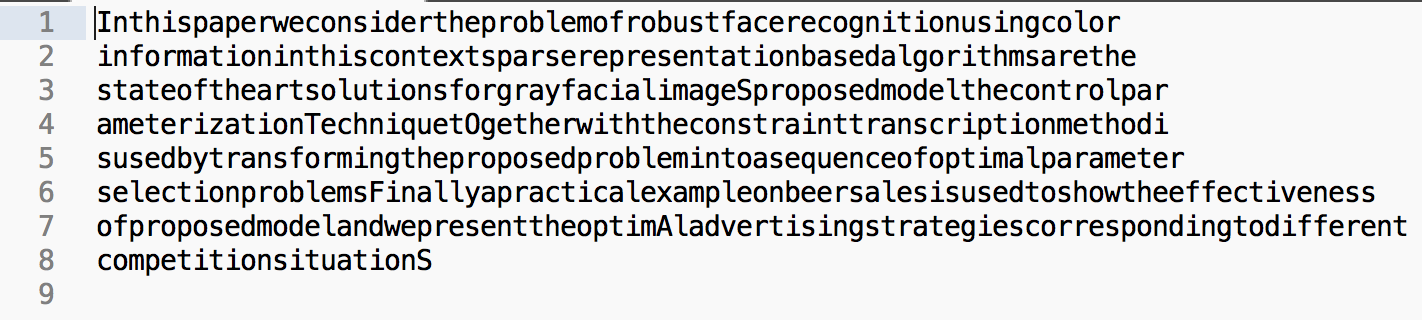
\includegraphics[width=\textwidth]{affine_plaintext.png}
	\caption{Original Plaintext File}
	\centering
\end{figure}

\begin{figure}[H]
	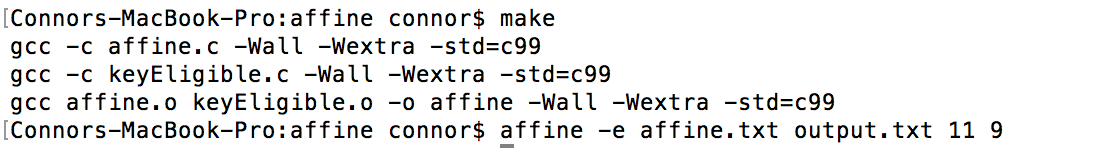
\includegraphics[width=\textwidth]{affine_encrypt.png}
	\caption{Encryption Process}
	\centering
\end{figure}

\begin{figure}[H]
	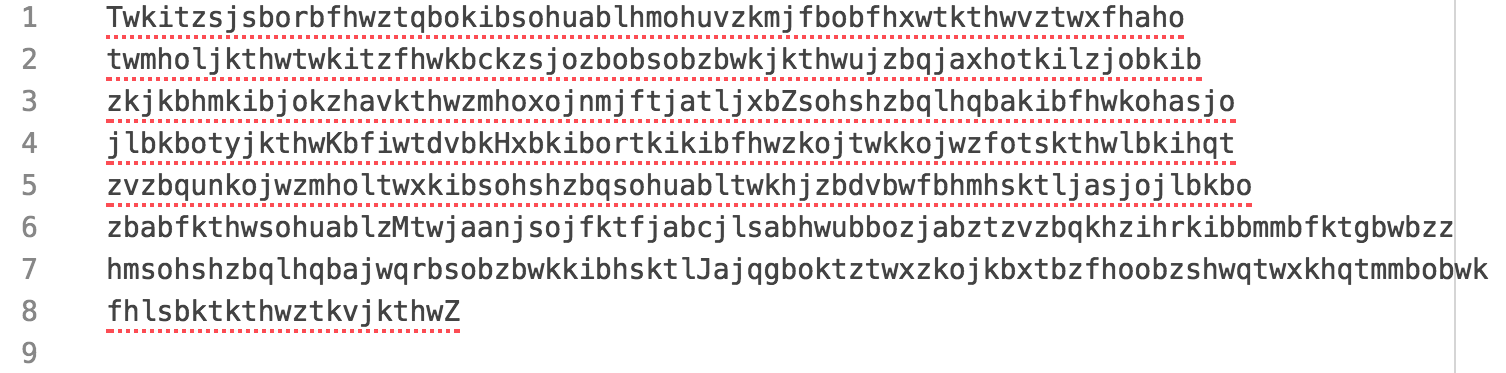
\includegraphics[width=\textwidth]{affine_ciphertext.png}
	\caption{Encrypted Ciphertext File}
	\centering
\end{figure}

\begin{figure}[H]
	
\includegraphics[width=\textwidth]{affine_decrypt.png}
	\caption{Decryption Process}
	\centering
\end{figure}

\begin{figure}[H]
	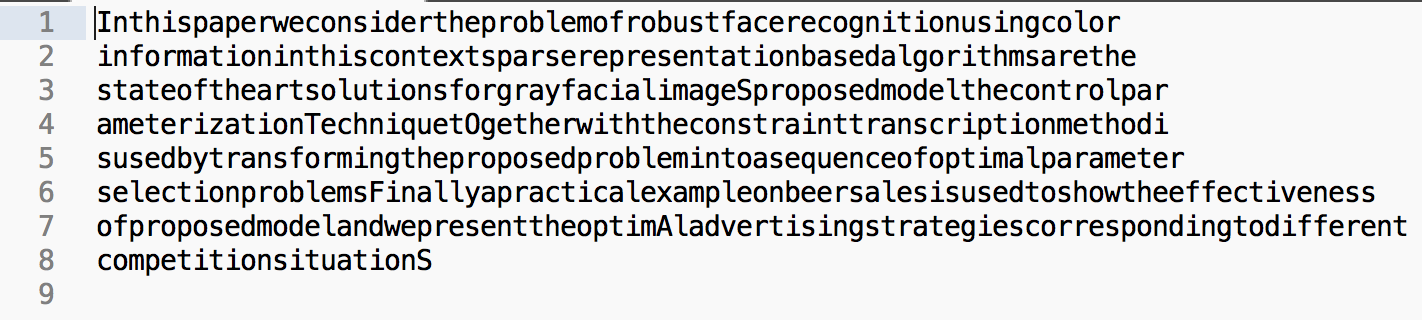
\includegraphics[width=\textwidth]{affine_plaintext.png}
	\caption{Recovered Plaintext file}
	\centering
\end{figure}

\section*{Affine Mathematical Proof}

The encryption and decryption functions for the affine cipher are as follows:

$$E(x)=(ax+b)\;mod\;m$$

$$D(x)=a^{-1}(x-b)\;mod\;m$$

\section*{Letter Distribution}

For the given test file shown in Figure 1, Figure 6 illustrates the letter distributions plotted via GNUPlot.


\break
%-------------------------------------------------------------------------------
% S-DES ENCRYPTION

\vspace*{-0.8cm}
\begin{center}
	\section*{S-DES}
\end{center}

\vspace*{0.8cm}
\section*{S-DES Mathematical Proof}

hello

\section*{Pseudo Code Structure}

hello

\section*{Encrypted Test File}

hello

\section*{Decrypted Test File}

hello

\section*{Utilization of an all 1 Key}

hello

\section*{Modify S-Boxes}

hello

\break
%-------------------------------------------------------------------------------
% FINAL QUESTIONS

\vspace*{-0.8cm}
\begin{center}
	\section*{Follow up Questions}
\end{center}

\vspace*{0.8cm}
\section*{Threats}

hello \\

\section*{Source Coding}

hello \\

\section*{Error Coding}

hello \\

\section*{S-DES Coding}

hello \\

\section*{S-DES Confusion and Diffusion}

hello \\

\break

%-------------------------------------------------------------------------------
\end{document}   
%-------------------------------------------------------------------------------